\documentclass{article}


% if you need to pass options to natbib, use, e.g.:
%     \PassOptionsToPackage{numbers, compress}{natbib}
% before loading neurips_2025

\PassOptionsToPackage{numbers, compress}{natbib}

% ready for submission
\usepackage{neurips_2025}


\bibliographystyle{abbrvnat}

\usepackage[pdftex]{graphicx}
\usepackage{amsmath}
% to compile a preprint version, e.g., for submission to arXiv, add add the
% [preprint] option:
%\usepackage[preprint]{neurips_2025}


% to compile a camera-ready version, add the [final] option, e.g.:
%     \usepackage[final]{neurips_2025}


% to avoid loading the natbib package, add option nonatbib:
%    \usepackage[nonatbib]{neurips_2025}


\usepackage[utf8]{inputenc} % allow utf-8 input
\usepackage[T1]{fontenc}    % use 8-bit T1 fonts
\usepackage{hyperref}       % hyperlinks
\usepackage{url}            % simple URL typesetting
\usepackage{booktabs}       % professional-quality tables
\usepackage{amsfonts}       % blackboard math symbols
\usepackage{nicefrac}       % compact symbols for 1/2, etc.
\usepackage{microtype}      % microtypography
\usepackage{xcolor}         % colors

\newcommand\reynotes[1]{\textcolor{purple}{#1}}

\title{SmokeViz: Using Pseudo-Labels to Develop a Human-Labeled Deep Learning Dataset of Wildfire Smoke Plumes in Satellite Imagery}

% The \author macro works with any number of authors. There are two commands
% used to separate the names and addresses of multiple authors: \And and \AND.
%
% Using \And between authors leaves it to LaTeX to determine where to break the
% lines. Using \AND forces a line break at that point. So, if LaTeX puts 3 of 4
% authors names on the first line, and the last on the second line, try using
% \AND instead of \And before the third author name.


\author{%
  Rey Koki\\%\thanks{rey.koki@colorado.edu} \\
  Department of Computer Science\\
  University of Colorado Boulder\\
  Boulder, Colorado 80303\\
  \texttt{rey.koki@colorado.edu} \\
  % examples of more authors
  % \And
  % Coauthor \\
  % Affiliation \\
  % Address \\
  % \texttt{email} \\
  % \AND
  % Coauthor \\
  % Affiliation \\
  % Address \\
  % \texttt{email} \\
  % \And
  % Coauthor \\
  % Affiliation \\
  % Address \\
  % \texttt{email} \\
  % \And
  % Coauthor \\
  % Affiliation \\
  % Address \\
  % \texttt{email} \\
}


\begin{document}


\maketitle


\begin{abstract}
    The global rise in wildfire frequency and intensity over the past decade underscores the need for improved fire monitoring techniques. To advance deep learning research on wildfire detection and its associated human health impacts, we introduce \textbf{SmokeViz}, a large-scale machine learning dataset of smoke plumes in satellite imagery. The dataset is derived from expert annotations created by smoke analysts at the National Oceanic and Atmospheric Administration, which provide coarse temporal and spatial approximations of smoke presence. To enhance annotation precision, we propose \textbf{pseudo-label dimension reduction (PLDR)}, a generalizable method that applies pseudo-labeling to refine datasets with mismatching temporal and/or spatial resolutions. Unlike typical pseudo-labeling applications that aim to increase the number of labeled samples, PLDR maintains the original labels but increases the dataset quality by solving for intermediary pseudo-labels (IPLs) that align each annotation to the most representative input data. For SmokeViz, a parent model produces IPLs to identify the single satellite image within each annotations time window that best corresponds with the smoke plume. This refinement process produces a succinct and relevant deep learning dataset consisting of over 180,000 manual annotations. The SmokeViz dataset is expected to be a valuable resource to develop further wildfire-related machine learning models and is publicly available at \reynotes{[aws download link]}.  
\end{abstract}


\section{Introduction}

Due in part to public policy, average fine particulate matter (PM\textsubscript{2.5}) levels in the US have generally declined over the past few decades \cite{clean_air_act}. Despite those improvements, the contribution of wildfire smoke to PM\textsubscript{2.5} concentrations in the US has more than doubled between 2010 to 2020, accounting for up to half of overall PM\textsubscript{2.5} exposure in Western regions \cite{smoke_PM}. Increases in PM\textsubscript{2.5} are a concern since ambient PM\textsubscript{2.5} exposure is a leading environmental risk factor for adverse health outcomes and premature mortality \cite{smoke_mortality}. These risks highlight the urgent need for effective wildfire monitoring methods to mitigate associated health impacts. 

Without the use of satellite remote sensing, wildfire monitoring has relied on ground-based methods, such as forest service patrols, manned lookout towers, and aviation surveillance \cite{smoke_monitoring}. While these methods provide valuable localized insights, they are constrained by geographical and logistical limitations, often failing to deliver timely and comprehensive data, especially over large and remote areas. In contrast, satellite imagery offers continuous, wide-area coverage and real-time streaming information critical for assessing the extent and movement of wildfire smoke.

Modern satellite sensors such as the Advanced Baseline Imager (ABI) aboard the Geostationary Operational Environmental Satellites (GOES) \cite{goes}, have revolutionized environmental monitoring. Unlike polar-orbiting satellites like Suomi or Sentinel, geostationary satellites provide persistent observation over fixed regions, essential for tracking the dynamic behavior of wildfire smoke plumes. GOES capabilities enables effective observations of smoke particulate concentration and movement, facilitating real-time air quality assessments.

Integrating satellite data into wildfire smoke monitoring can improve the responsiveness of public health interventions. Mapping the spread and density of smoke allows health authorities to issue timely warnings, initiate evacuation protocols, and allocate resources efficiently. Moreover, historical satellite records can help researchers understand the broader impacts of wildfire smoke, informing policy decisions and mitigation strategies.

In addition, numerical models used for real-time smoke dispersion lack a dedicated smoke analysis product available for data assimilation \cite{hrrr, rrfs}. This absence leads to delayed model spin-up and propagates errors in the forecasts. A satellite-driven, real-time smoke assimilation product could significantly decrease the computational requirements and enhance the accuracy of existing smoke dispersion models. 

\section{Related Work}

\subsection{Numerical}

Currently, multi-channel thresholding is a popular method to distinguish smoke pixels from pixels containing dust, clouds or other phenomenon with similar signatures \cite{threshold}. Thresholds are determined by using historical, labeled data to extract optimal radiance values for each channel that corresponds with the labeled class. These methods are tuned to particular biogeographies and often have issues with generalization to new locations with varying fuel types \cite{thresh_geog}.

\subsection{Analyst} 
In contrast to the numerical thresholding approach, human visual inspection of satellite imagery is another commonly used method for smoke identification. Trained analyst inspect satellite imagery and label the smoke by hand. An example of hand-labeled annotations is the National Oceanic and Atmospheric Administration (NOAA) Hazard Mapping System (HMS) fire and smoke product \cite{hms, hms_val}. For the HMS smoke product, trained satellite analysts use movement characteristics to help identify smoke by scanning through a time series of satellite imagery. When visual inspection indicates smoke, the analyst will draw a polygon that corresponds to the geolocation and density of smoke. By design of the product, the HMS annotations have varying time resolution and are released on a rolling but undefined schedule ranging from one to multiple times a day as observation conditions permit. If expanded beyond the current North American boundary, this method will not be as scalable as an automated approach and is limited by the availability of analysts and their time. 

The HMS program, managed by NOAA, consists of an operational system that uses an aggregation of satellite data to generate active fire and smoke data. To train our model, we develop a supervised learning framework that uses the HMS analyst smoke product as truth labels during the model training process. HMS smoke analysis data gives the coordinates of the smoke perimeter as a polygon and classifies the smoke by density within a given time window. The time windows can range from instantaneous (same start/end time) to lengths of 22 hours. While the true bounds of the smoke can change within the larger time spans, the analyst is making an approximation that should reflect the smoke coverage over the duration of the time window. The density information is qualitatively determined by each analyst based on the apparent smoke opacity in the satellite imagery and categorized as either light, medium or heavy as seen in figure \ref{densities}a \cite{hms_web}.

\subsection{Deep Learning}

To address the challenges associated with thresholding and manual labels, we can look towards innovative approaches and recent technological advancements in computer vision. Machine learning methods have shown potential in improving the accuracy and efficiency of satellite-based wildfire smoke detection and monitoring. For instance, SmokeNet, uses a convolutional neural network (CNN) based framework to determine if a scene of MODIS satellite imagery contains smoke \cite{smokenet}. Another study, that looked at a singular wildfire event, also used a CNN to identify smoke on a pixel-wise basis using imagery from Himiwari-8 \cite{larsen}. Additionally, Wen et al. developed a CNN architecture that takes GOES-East imagery as input and the HMS-generated annotations for the target labels during training \cite{smoke_goes}. Contrary to previous GOES-based machine learning datasets that include data from only one of the two operational GOES-series satellites, most commonly opting for GOES-East \cite{smoke_goes, wildfire_detect, goes_conv, contrail}, the annotations in SmokeViz are matched with either GOES-East or GOES-West based on which satellite has optimal coverage of the event. 

The success of deep learning methods, such as CNNs, relies heavily on the availability of a large, representative dataset \cite{data_size}. As laid out in table \ref{studies}, prior studies use relatively small numbers of samples, where one sample represents a satellite image with a singular time and geolocation. In contrast, benchmark datasets for computer vision applications contain tens of thousands (CIFAR-10 \cite{cifar} and MNIST \cite{mnist}) to millions (CIFAR-100 and ImageNet \cite{imgnet}) of data samples \reynotes{compare to large remote sensing datasets}. Keeping in mind the correlation between both the quality and quantity of data with model performance, we introduce the largest known smoke plume dataset, SmokeViz, containing over 180,000 samples.

\begin{table*}[h]
    \caption{Comparison of satellite smoke plume datasets detailing the number of samples containing smoke, observational satellite, number of bands/channels included, how the labels were generated and whether the labels are for image scene classification (SC) or semantic segmentation (SS)and if the dataset is publicly available.}\label{studies}
    \centering
    \begin{tabular}{ccccrrcrc}
        \toprule
        reference & \verb|#| samples & satellite & \verb|#| bands & label & task & avail.\\
        \midrule
        \cite{smokenet}& 1016 & MODIS & 5 & students & SC & no \\
        \cite{smoke_goes}& 4095 & GOES-East & 5 & HMS analysts & SS & no \\
        \cite{larsen} & 975 & Himiwari-8 & 7 & algorithm& SS & no \\
        %Smoke-Unet \cite{wang}& 47 & Landsat-8 & 4 & segmentation & \\
        \cite{satlas} & 125 & Sentinel-2 & 3 & crowd sourced & SC & yes \\
        SmokeViz  & 183,672 & GOES-East/West & 3 & HMS analysts & SS & yes \\
        \bottomrule
    \end{tabular}
\end{table*}

Semi-supervised learning is an approach that can be used to increase the number of labeled samples in a dataset. This is performed by leveraging a labeled dataset to generate new labels for an often larger, but unlabeled, dataset. Pseudolabeling, a form of semisupervised learning, is an iterative process that uses labeled data to train an initial parent model. The parent model is applied to unlabeled data to create pseudo-labels (PL) that are then used to train a child model; if performed iteratively, the child model will then create another round of PLs to train the next child model \cite{pseudo}. We introduce a noniterative variation of pseudo-labeling, not to increase the size, but to reduce the noise and thus dimensionality of our dataset. This is done by generating intermediary PLs (IPLs) that are not used to train models, but will serve as a tool to select the optimal satellite image out of the given time window to best represent each smoke plume analyst annotation. The final resulting dataset, SmokeViz, is comprised of expert smoke-specific analyst annotations of wildfire smoke plumes and the corresponding GOES satellite imagery.

Although the SmokeViz dataset is expected to be primarily used to solve various wildfire smoke applications, the dataset has the potential to serve as a uniquely insightful test case for remote sensing semantic segmentation. Many existing remote sensing datasets have removed imagery with clouds \cite{bigearthnet, crops} and/or are focused on objects with sharp contrasts such as crops \cite{crops}, human infrastructure \cite{polyworld}, or clouds over oceans \cite{cyclone, cloud_texture}, smoke has indistinct boundaries that often fade both spatially and temporally. Adding difficult to curate, high quality remote sensing specific datasets like SmokeViz to large-scale multi-category pretraining datasets such as SatlasPretrain \cite{satlas} has the potential to advance generalizable remote sensing computer vision.

\begin{figure}[!htb]
    \centering
    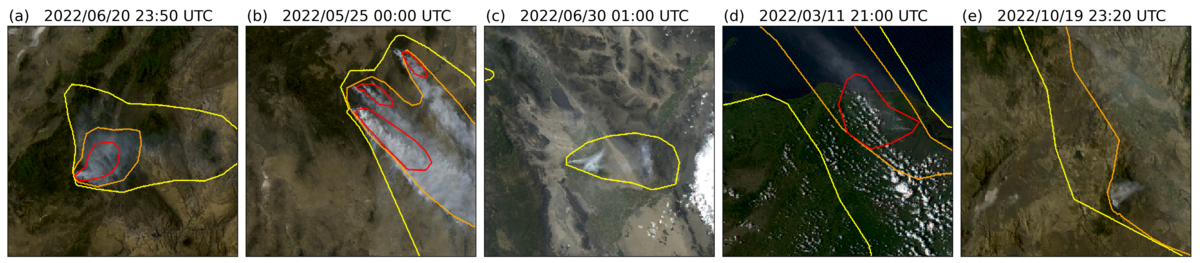
\includegraphics[width=\linewidth]{figures/variations_small.png}
    \caption{HMS smoke annotations overlaid on GOES imagery, the yellow, orange and red contours indicate the extent of light, medium and heavy density smoke. (a) and (b) show a canonical examples of a smoke plumes. (c)-(e) show observable variations in the density labels.}\label{densities}
\end{figure}

\section{Methods}
\subsection{Datasets}

The smoke plumes in our datasets are observed using the latest GOES operational satellites, GOES-16 (East), 17 and 18 (West) that each carry the ABI, which measure 16 bands between the visible and infrared wavelengths (\(\lambda\)s) collected every 10 minutes for full-disk imagery. Using PyTroll, a Python framework for processing satellite data \cite{satpy}, we input bands 1-3 (Table \ref{rgb_bands}) to a GOES-specific true color composite algorithm \cite{true_color} to develop a 1km resolution true color image representation, similar to the imagery seen by HMS analysts. Discussed in further detail in the next section, we only include the first 3 of 16 available bands due the smaller \(\lambda\)s of light corresponding to the highest signal-to-noise ratio (SNR).

To take into account movement characteristics to help identify smoke, analysts use multi-frame animations of the satellite imagery. The resulting annotations primarily have time windows over multiple hours, with an average of 3 hours of imagery representing one smoke plume annotation. Since the goal of HMS smoke annotations is to show the general coverage over that time span, as shown in figure \ref{timelapse}, the smoke boundaries don't often match up with the satellite imagery over the entire time window. One approach to this problem would be to use all the satellite images the analysts used as input. Since the timespans are non-uniform, this would vary the length in imagery inputs into the model, which would be difficult with a CNN architecture. Moreover, this would result in a smoke plume detection model that ingests a longer sequence of start-up imagery that requires additional memory and computational resources than a single input image. Instead of using the original analysts' many satellite image inputs to one annotated output, we develop a one-to-one input-to-output by identifying the optimal singular satellite image input to represent each analyst annotation. 

\begin{figure}[!htb]
    \centering
    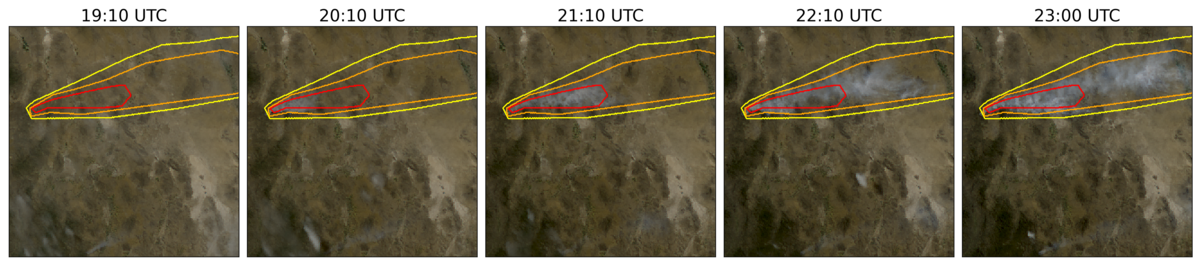
\includegraphics[width=\linewidth]{figures/timelapse_small.png}
    \caption{True color GOES-East imagery from May 5th, 2022, Southeast New Mexico (\(31.38^{\circ}\)N, \(107.87^{\circ}\)W) during the start of the Foster Fire. The red, orange and yellow lines represent the heavy, medium and low density HMS smoke annotations that span 19:10\textendash23:00 UTC.}
    \label{timelapse}
\end{figure}

As mentioned prior, rather than using one satellite or the cumulative data from both GOES-West and GOES-East images, we select between one or the other satellite based on the solar zenith angle (SZA). For smoke identification, this approach can achieve a much higher SNR than imaging the earth’s surface from an arbitrary angle. While the atmosphere is composed primarily of molecules with size \(<\)1nm, smoke particles are larger in comparison, varying from 100 nm -- 10 \(\mu\)m in diameter, \(d\). When the \(\lambda\) of light \(\lambda<d\), the elastic scattering of light against matter is modeled through Mie rather than Rayleigh scattering (figure \ref{mei}) which contributes to two critical consequences: (1) the forward scattering light that travels colinearly from sun to smoke, to satellite will have the highest SNR as seen in subfigures \ref{WEST_EAST_bands}(a) vs \ref{WEST_EAST_bands}(b) that show GOES-East providing a higher SNR near sunset compared to GOES-West. (2) The smaller the \(\lambda\) in relationship to \(d\), the higher the smoke SNR, as seen in subfigures \ref{WEST_EAST_bands}(c)-\ref{WEST_EAST_bands}(e). In order to balance the need for a representative, information dense dataset that remains a manageable size to host online, we use the Mie scattering physics principles to narrow down our dataset. (1) we choose imagery from GOES-East or GOES-West that would be able to observe the highest smoke related forward scattering. (2) we choose the three ABI bands with the smallest available \(\lambda\), 0.47\(\mu\)m, 0.64\(\mu\)m and 0.865 \(\mu\)m (C01-C03). 


\begin{figure}[!htb]
    \centering
    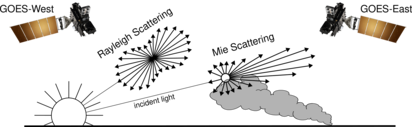
\includegraphics[width=8cm]{figures/mei_small.png}
    \caption{If the particle size is \(<\frac{1}{10}\) the \(\lambda\) of the interacting light, then the primary scattering will be Rayleigh. Mie scattering is the predominant scattering mechanism when the particle size is larger than the \(\lambda\) of light. This schematic demonstrates that when the sun is setting in the West, the Mie scattering will predominately forward scatter towards GOES-East.} \label{mei}
\end{figure}

For the existing dataset of HMS smoke plume annotations and all corresponding satellite imagery, \(\mathcal{D} = \{\mathcal{X}, \mathcal{Y}\}\), for each sample, a label \(y_i \in \mathcal{Y}\) has a set of satellite imagery \([x_{(i,t_0)},...,x_{(i,t_N)}] \in \mathcal{X}\) over the analyst defined time window \(t\). To develop a one-to-one data-to-label dataset, we generate IPLs to develop a subset of \(\mathcal{D}\), denoted as \(\mathcal{D}_p\), that has a one-to-one ratio such that \(|\mathcal{X}_p| = |\mathcal{Y}|\), where we aim to find the satellite image that has the maximum overlap between the geolocation of smoke in the imagery and the analyst annotation using the PLDR method shown in figure \ref{PLDR}.

\begin{figure}[!htb]
    \centering
    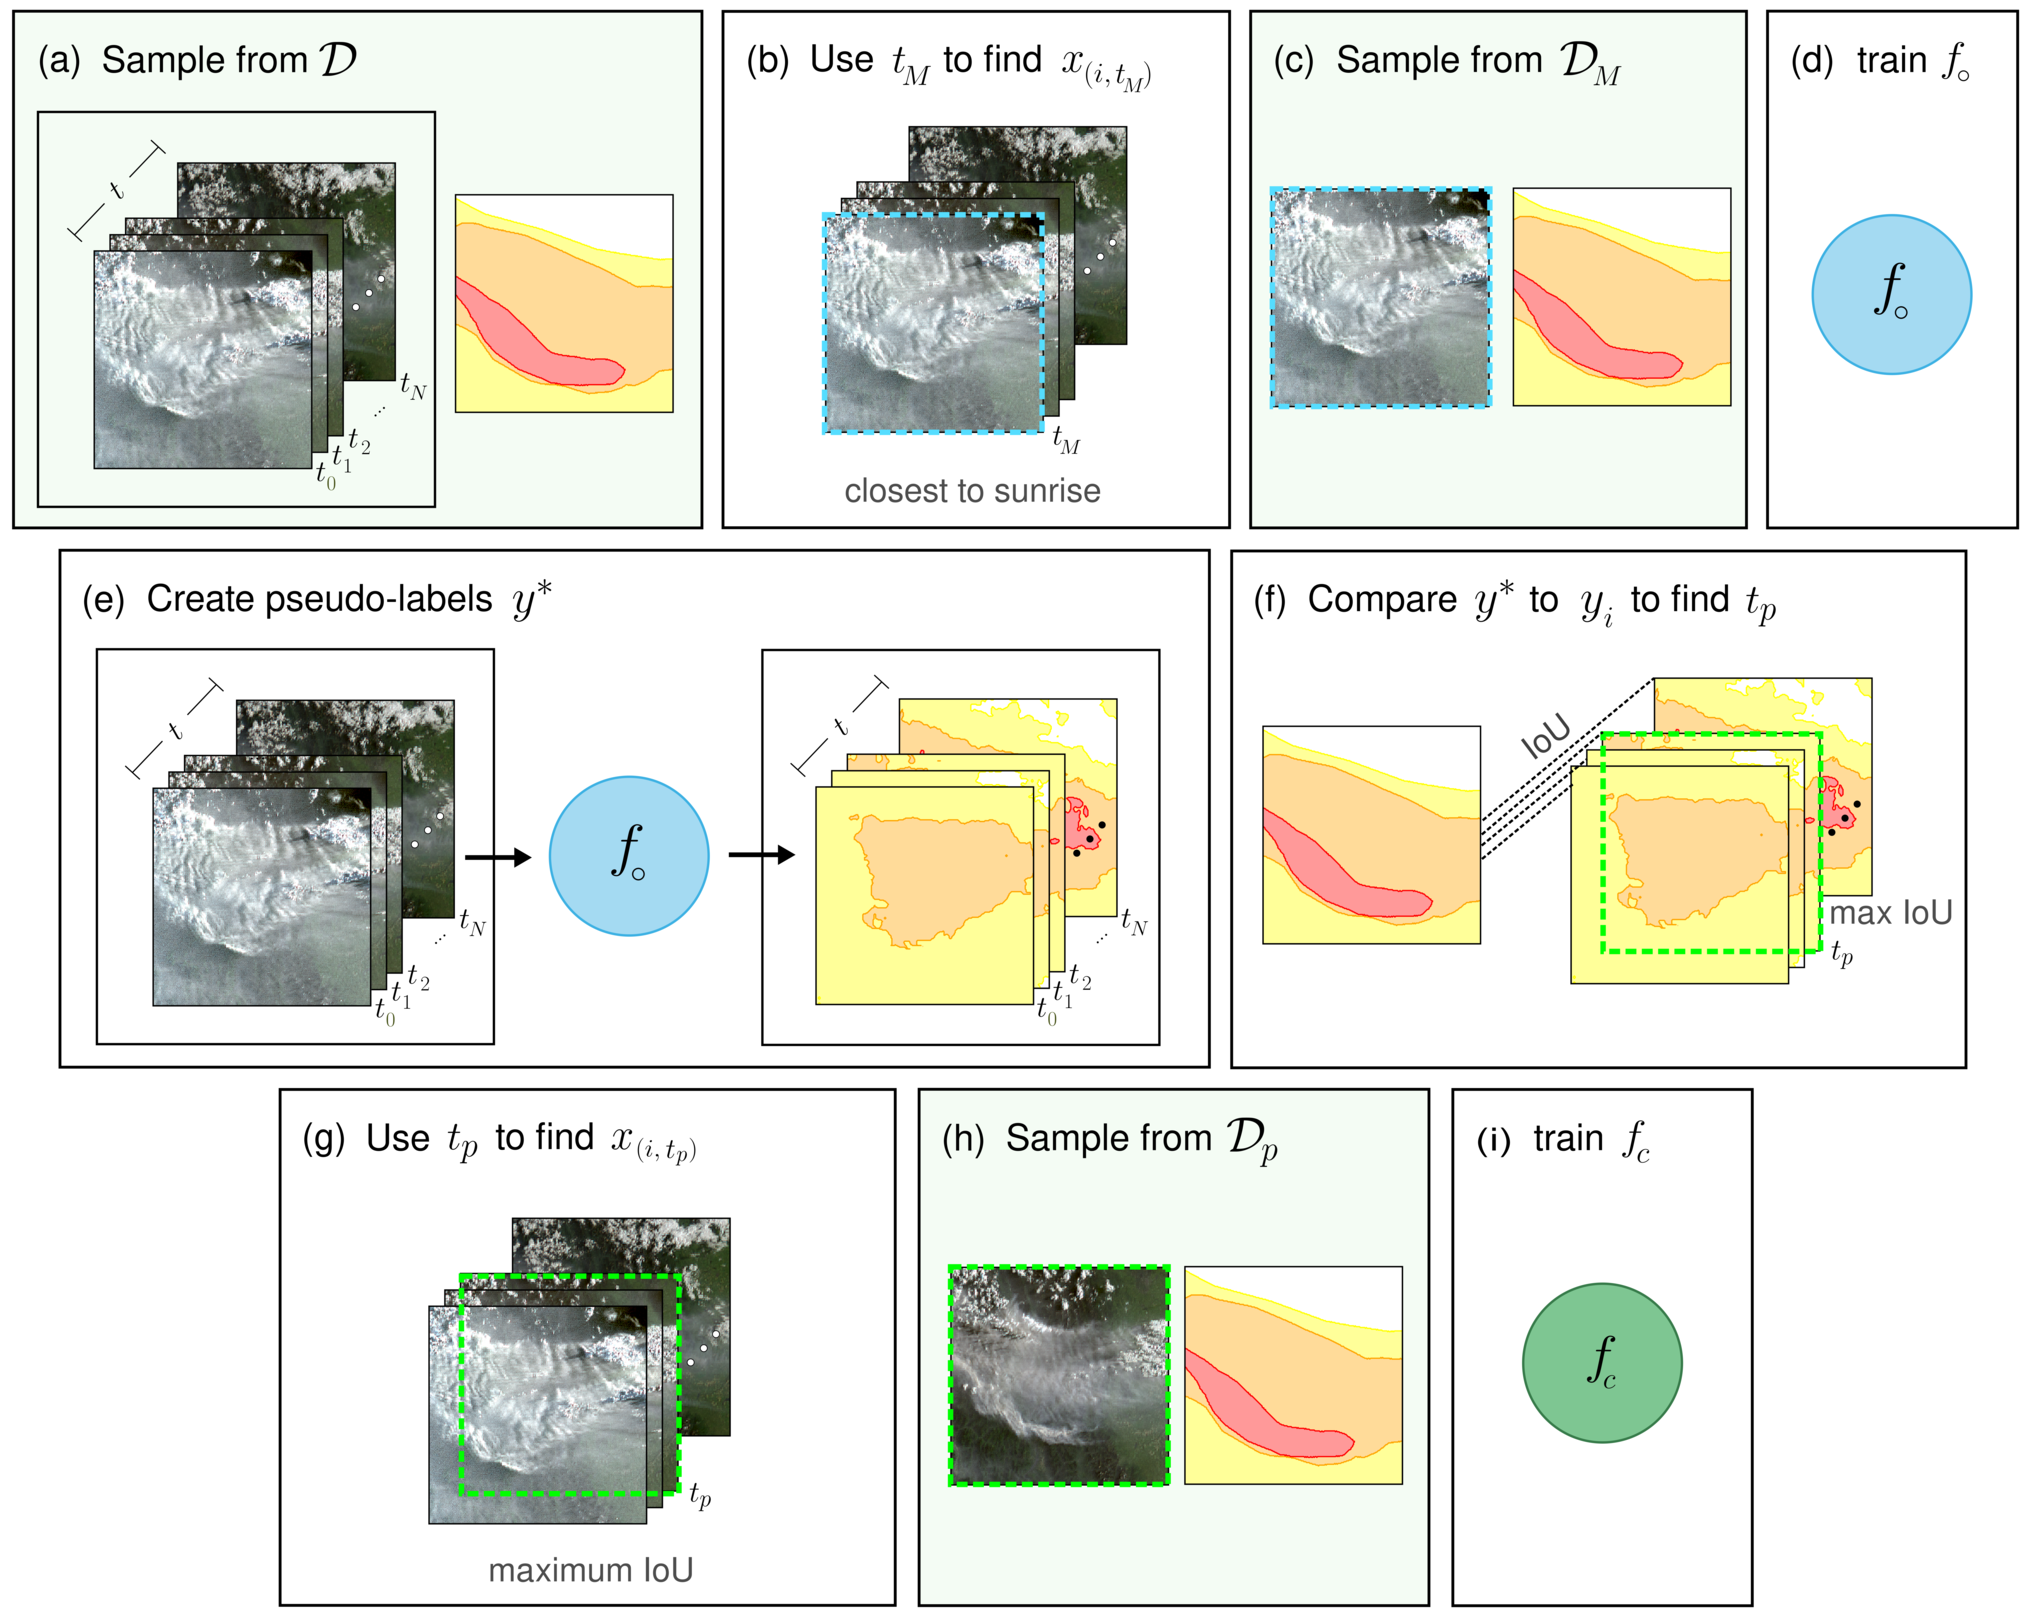
\includegraphics[width=\linewidth]{figures/workflow_small.png}
    \caption{PLDR applied to create the SmokeViz dataset, the green boxes represent the dataset stages, note that the HMS analyst label \(y\) remains the same, the only change is for the satellite image(s) \(x\). (a) for a sample in the original full dataset \(\mathcal{D}\), each analyst annotation \(y_i\) corresponds to \(N\) satellite images that cover time window \(t\) so that \(([x_{(i,t_0)},...,x_{(i,t_N)}], y_i) \in \mathcal{D}\) (b) using Mie scattering physics we find the satellite image, \(x_{(i,t_M)}\) that correlates with the time, \(t_M\), that would produce the highest possible SNR if smoke was present (c) the resulting \(\mathcal{D}_M\) has a one-to-one ratio of image-to-annotation \((x_{(i,t_M)}, y_i) \in \mathcal{D}_M\) (d) use \(\mathcal{D}_M\) to train the parent model, \(f_\circ(x_{(i,t_M)})=y_i\) (e) apply a greedy algorithm \(f_\circ([x_{(i,t_0)},...,x_{(i,t_N)}])=[y^*_{(i,t_0)},...,y^*_{(i,t_N)}]\) to create IPLs \(y^*\) for each candidate image (f) use the intersection over union (IoU) metric to compare \(y^*\) to the analyst annotation, \(y_i\), and identify the time, \(t_p\), where the IPL and analyst annotation have the maximum IoU (g) use the time of highest overlap between \(y^*\) and \(y_i\) to identify the sample, \(x_{(i,t_p)}\), that should best match the analyst annotation (h) \(\mathcal{D}_p\) has a one-to-one ratio of image-to-annotation \((x_{(i,t_p)}, y_i) \in \mathcal{D}_p\) (i) use the SmokeViz dataset \(\mathcal{D}_p\) to train deep learning models \(f_c(x_{(i,t_p)})=y_i\) to detect and classify the density of wildfire smoke plumes in GOES imagery.}\label{PLDR}
\end{figure}

To train an initial parent model, \(f_{\circ}\), we developed a method of leveraging Mie scattering physics to select \(x_{(i,t_M)} \in \mathcal{X}\) (figure \ref{PLDR}(b)) so that \(x_{(i,t_M)}\) has a higher chance than random selection out of the set of imagery \([x_{(i,t_0)},...,x_{(i,t_N)}]\) to be representative of \(y_i\). This Mie-Derived Dataset, \(\mathcal{D}_M\) produces a training set so that if there is smoke present during the entire time window, the selected timestamp \(t_M\) would give the highest smoke SNR. 

More importantly than finding the timestamp for maximum the SNR, we want to determine which image actually has smoke present within the smoke label boundaries. We use \(\mathcal{D}_M\) to train \(f_{\circ}\) (figure \ref{PLDR}(d)), to identify smoke in satellite imagery, and then use that \(f_{\circ}\) to create IPLs of each satellite image in a given annotation's time-window (figure \ref{PLDR}(e)). From those results, the optimal satellite image is chosen based on which image's IPLs has the greatest overlap with the analyst annotation (figure \ref{PLDR}(f)-(h)).


\subsubsection{Mie-Derived Dataset \(\mathcal{D}_M\)}

We apply a physics-based approach to select the Mie-derived dataset, \(\mathcal{D}_M\), from the full dataset \(\mathcal{D}\), so that \(\mathcal{D}_M \subset \mathcal{D}\) and so that \(|\mathcal{X}_M|=|\mathcal{Y}|\) so that we can efficiently and effectively train \(f_o\). Based on the criteria to optimize for maximum observation of Mie forward scattering, the trivial strategy would be to pull imagery from GOES-West right after sunrise and from GOES-East right before sunset when the SZA is \(90^{\circ}\). However, the time when the SZA approaches \(90^{\circ}\) coincides with when there are maximized atmospheric interactions that cause an increase in noise and artifacts \cite{zen_angle}. With the goal to reduce large SZA related noise, when there are multiple frames to choose from, we choose the image with the largest SZA that is \(<88^{\circ}\).

The Mie-derived image selection process accounts for atmospheric properties and light scattering physics to calculate which singular satellite image within the analyst time-window could give the highest possible smoke SNR if smoke was equally present throughout the time-window. The resulting Mie-derived dataset, \(\mathcal{D}_M = \{\mathcal{X}_M, \mathcal{Y}\}\), contains over 200,000 samples and was then used to train a parent model, \(f_{\circ}\). 




\begin{figure}[!htb]
    \centering
    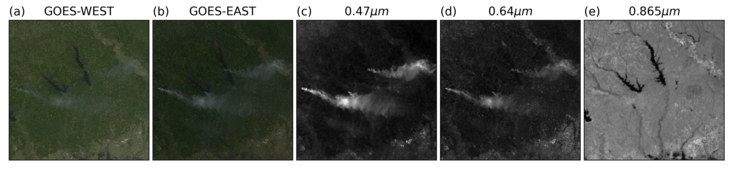
\includegraphics[width=\linewidth]{figures/GOES_WEST_EAST_B_R_V_small.png}
    \caption{True color (a) GOES-WEST and (b) GOES-EAST imagery from March \(23^{rd}\), 2022 centered at (\(31.1^{\circ}\), \(-93.8^{\circ}\)) in Texas, USA taken at 23:20 UTC. The GOES-EAST raw band imagery for (c) blue, (d) red and (e) veggie bands show variations in the SNR for smoke detection in relation to the \(\lambda\) of light being measured.}\label{WEST_EAST_bands}
\end{figure}

\subsubsection{PLDR Dataset \(\mathcal{D}_p\)} 

To build the deep learning architecture for \(f_o\) we use the high level API package Segmentation Models Pytorch \cite{semantic} to implement EfficientNetV2 \cite{efficientnetv2} as the encoder with random initialized weights connected to the semantic segmentation classifier from the PSPNet model \cite{pspnet}. The data input is 256x256x3 snapshots of 1km resolution true color GOES imagery that contain smoke and output a 256x256x3 classification map that predicts if a pixel contains smoke and if so, what the categorical density of that smoke is. Since the smoke density labels are ordinal, we apply the thermometer encoding shown in table \ref{therm} to encode the smoke densities and apply binary cross entropy as the loss function per density of smoke. 



\begin{table}
\parbox{.45\linewidth}{
\centering
    \caption{A comparison of how smoke density would be represented by one-hot encoding commonly used for categorical data to thermometer encoding often used for ordinal data.}\label{therm}
    \begin{tabular}{ccccrrcrc}
        \toprule
        density & one-hot & thermometer \\
        \midrule
        none & \texttt{[0 0 0]} & \texttt{[0 0 0]} \\
        light  & \texttt{[0 0 1]} & \texttt{[0 0 1]} \\
        medium & \texttt{[0 1 0]} & \texttt{[0 1 1]} \\
        heavy  & \texttt{[1 0 0]} & \texttt{[1 1 1]} \\
        \bottomrule
    \end{tabular}
}
\hspace{.4cm}
\parbox{.5\linewidth}{
    \caption{Dataset split for \(\mathcal{D}_M\) and \(\mathcal{D}_p\), samples for 2024 go up to November 1st \reynotes{do 2018-2022 instead}. We use an entire year of data for both validation and testing sets to capture year-long wildfire trends.}\label{split}
    \centering
    \begin{tabular}{ccccrrcrc}
        \toprule
        dataset & \(\mathcal{D}_M\) & \(\mathcal{D}_p\) &years\\
        \midrule
        training & 165,609 & 144,225 &2018-22\\
        validation & 20,056 & 19,223 &2023 \\
        testing & 21,541 & 20,224 & 2022 \\
        \bottomrule
    \end{tabular}
}
\end{table}

To determine which image out of the relevant imagery for the given time window best represents the analyst annotation, we implement a greedy algorithm (figure \ref{PLDR}(e)) \(f_\circ([x_{(i,t_0)},...,x_{(i,t_N)}])=[y^*_{(i,t_0)},...,y^*_{(i,t_N)}]\). The outputs of \(f_{\circ}\), \([y^*_{(i,t_0)},...,y^*_{(i,t_N)}]\) give \(N\) predictions on the location and density of smoke in the imagery over the analyst defined time window \(t\). Each \(y^*\) serve as a semantic segmentation IPL of smoke and are compared to the corresponding analyst annotation, \(y_i\). To compare each \(y^*\) to \(y_i\) (figure ref{PLDR}(f)), we calculate the intersection over union (IoU) using the total set of pixels for \(y^*\) at that density of smoke and the entire set of pixels for \(y_i\) for a particular smoke density in each image as shown in equation \ref{overall_iou}. The timestamp, \(t_p\) associated with the IPL with the highest IoU score, \(y^*_{(i,t_p)}\) is matched to the corresponding image, \(x_{(i,t_p)}\) (figure \ref{PLDR}(g)), that is predicted to best represent the analyst smoke annotation, \(y_i\). A standard implementation detail for PLs \cite{conf_thresh}, a confidence threshold value is defined to determine if the corresponding sample (\(x_{(i, t_p)}, y_i\)) should to be included in the dataset \(\mathcal{D}_p\). Based on subjective visual inspection by the authors of when the satellite imagery became consistently unidentifiable to its label, we chose a confidence threshold that would include the sample in \(\mathcal{D}_{p}\) if the maximum overall IoU was over 0.01. 
\reynotes{say size}

\begin{equation} \label{overall_iou}
    IoU_{\text{overall}} = \frac{\sum\limits_{j=\text{light}}^{\text{heavy}}|y_{j}\cap y^*_{j}|}{\sum\limits_{j=\text{light}}^{\text{heavy}}|y_{j}|\cup|y^*_{j}|}
\end{equation}



The same dataset split choices and model training setup that were used for \(\mathcal{D}_{M}\) and \(f_{\circ}\) were implemented for \(\mathcal{D}_p\) and \(f_c\). As depicted in figure \ref{PLDR}(e), we use \(\mathcal{D}_{p}\) to train a child model \(f_c\). To assess if training with \(\mathcal{D}_{p}\) can produce a more robust semantic segmentation model compared to training on \(\mathcal{D}_M\) we run \(f_c\) on the \(\mathcal{D}_{p}\) and \(\mathcal{D}_{M}\) test sets. 

\subsection{Benchmark Models}

We benchmark the SmokeViz dataset \(\mathcal{D}_{p}\) by varying the semantic segmentation classification heads. We train Linknet \cite{linknet}, PSPNet \cite{pspnet} and MANet \cite{manet} using the same encoder for \(f_c\) and \(f_{\circ}\), EfficientNetV2. Each model is trained over 100 epochs using a batch size of 32 and the Adam optimizer on 8 Nvidia P100 GPUs allocating 100GB of memory over 12 hours of allotted training time. We choose these architectures because of their abilities to capture multi-scale objects such the varying spatial extents of smoke plumes.

\section{Results}

To interpret the performance of \(f_{\circ}\), we report the IoU metrics in table \ref{iou_results} that were computed by running \(f_{\circ}\) and \(f_c\) on \(\mathcal{D}_M\) and \(\mathcal{D}_{p}\). For each density, we calculate the IoU using the total set of pixels that \(f_{\circ}\) predicts as that density of smoke and the entire set of pixels labeled by the analyst as a particular smoke density over all imagery contained in the testing dataset. Additionally, we compute the overall IoU for all densities by first computing the number of pixels that intersect their corresponding density and divide that by the total number of pixels that make up the union of model predicted and analyst labeled smoke in the testing dataset.

\begin{table} 
    \caption{IoU results per density of smoke and over all densities using \(f_{\circ}\) and \(f_c\) with \(\mathcal{D}_M\) and \(\mathcal{D}_p\).}\label{iou_results}
    \centering
    \begin{tabular}{lcc|cc}
        \toprule
        \multicolumn{1}{c}{} & \multicolumn{2}{c}{\(f_{\circ}\)} & \multicolumn{2}{c}{\(f_c\)}\\
        \midrule
        \multicolumn{1}{c}{} & \(\mathcal{D}_M\) & \(\mathcal{D}_{p}\) & \(\mathcal{D}_M\) & \(\mathcal{D}_{p}\) \\
        \midrule
        Heavy   & 0.278 & 0.368 & 0.218 &  0.411 \\
        Medium  & 0.310 & 0.417 & 0.319 &  0.484 \\
        Light   & 0.480 & 0.585 & 0.491 &  0.660 \\
        Overall & 0.430 & 0.533 & 0.438 &  0.607 \\
        \bottomrule
    \end{tabular}
\end{table}

\begin{figure*}
    \centering
    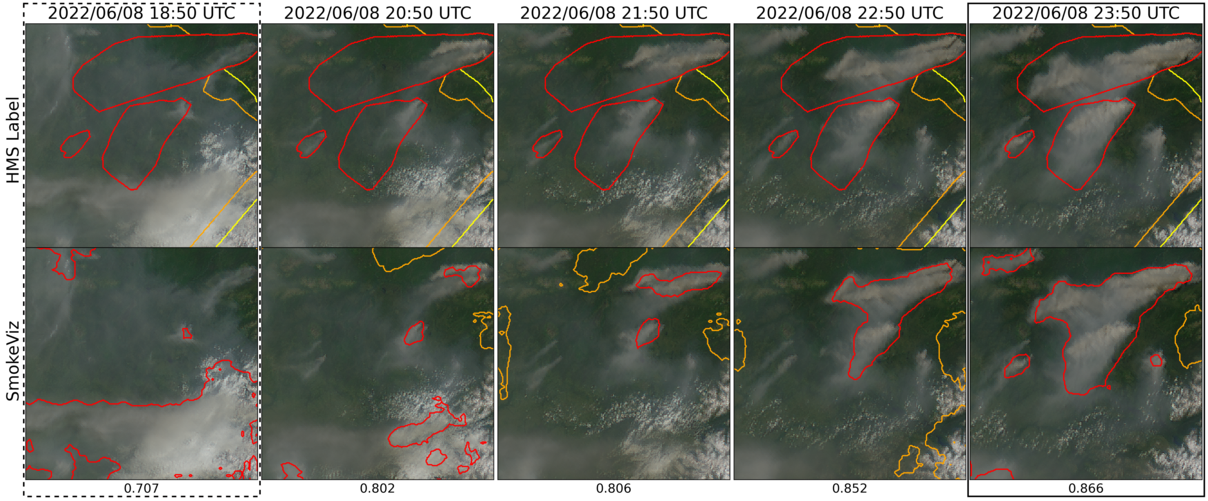
\includegraphics[width=\linewidth]{figures/final_results_small.png}
    \caption{GOES-West imagery showing smoke on June 8th, 2022 in Alaska where, at this geolocation (\(61.06^{\circ}\)N, \(156.12^{\circ}\)W), daylight was between 12:43-7:53 UTC. The HMS smoke annotations (top row) span from 18:50 to 23:50 UTC and are compared to the \(f_{\circ}\) generated pseudo-labels (bottom row). The first column (dotted outline) would be the GOES imagery selected for \(\mathcal{D}_{M}\) since it is closest to sunrise. The last column (solid outline) was selected for \(\mathcal{D}_{p}\) since it had the highest IoU value between the pseudo-label and analyst annotation. The IoU score over all densities is reported at the bottom of each column.}
    \label{ml_vs_mei}
\end{figure*}

An illustration of a pseudo-label picked image better representing the analyst annotation when compared to the Mie-derived image selection is evident in Figure \ref{ml_vs_mei}, where the heavy density smoke IoU increases from 0.01 to 0.59. The analyst annotation for these densities cover 5 hours of imagery, the Mie-derived selection optimizes for the image closest to sunrise while the pseudo-label image selection chooses the image with the highest overlap between the pseudo-label and the analyst annotation. The figure also illustrates how using a deep learning model can provide higher time resolution and give a dynamic representation of smoke over time.

To get an idea on how \(f_{c}\) compares to the HMS analyst annotations we show a series of samples from \(\mathcal{D}_{p}\) in figure \ref{bench}. The examples give a qualitative representation of how the predictions from \(f_c\) can provide more detailed boundaries of smoke densities than the HMS annotations do.

\begin{table}[h]
    \caption{Comparison of semantic segmentation model IoU performance on \(\mathcal{D}_{p}\).}\label{bench}
    \centering
    \begin{tabular}{cccrrcrc}
        \toprule
           & DLV3+ & MANet & PSPNet & Linknet \\
        \midrule
        heavy   & 0.411 & 0.336  & 0.355 & 0.324 \\
        medium  & 0.484 & 0.487  & 0.502 & 0.456 \\
        light   & 0.662 & 0.675  & 0.690 & 0.662 \\
        overall & 0.607 & 0.615  & 0.626 & 0.601 \\
        \bottomrule
    \end{tabular}
\end{table}

The results for the benchmarking models (table \ref{bench}) show similar performance across the models. DeepLabV3+ (\(f_c\)) gives the highest heavy density smoke IoU value, while PSPNet gives the highest overall IoU score.

\begin{figure}[!htb]
    \centering
    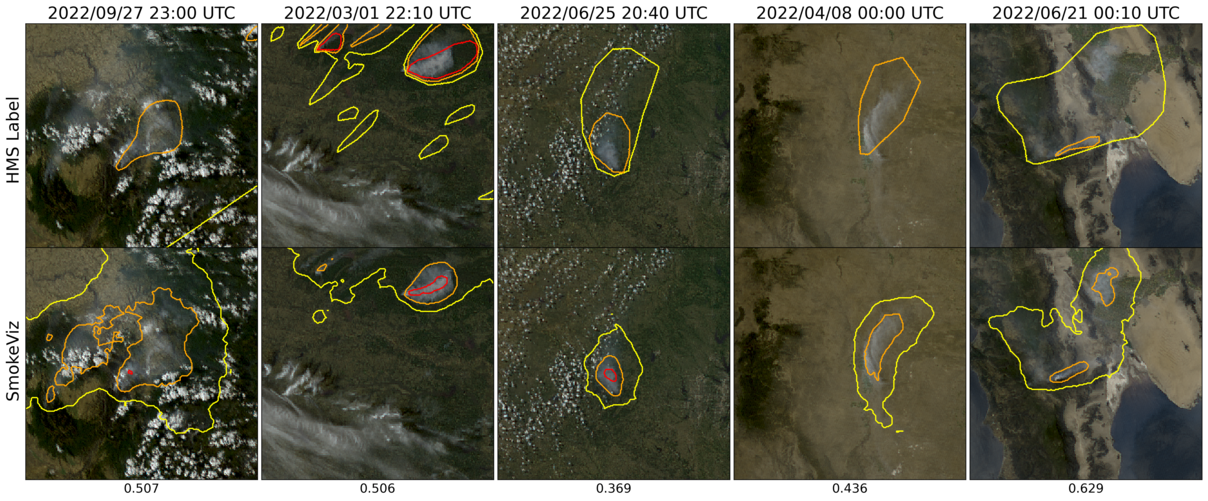
\includegraphics[width=\linewidth]{figures/examples_small.png}
    \caption{Examples of HMS annotations (top row) vs \(f_{c}\) output (bottom row) on \(\mathcal{D}_{p}\) samples. The overall IoU score is reported at the bottom of each column.}\label{examples}
\end{figure}

\section{Limitations}

One of the concerns that comes with using pseudo-labeling methods is that you can perpetuate biases from the parent model into subsequent child models. Due to the increase in detectable forward scattered light off smoke particular matter, we expect the model to have a bias towards producing a higher success rate for smoke detection at larger solar zenith angles. The original HMS annotations do not distinguish by type of fire and include a large representation of controlled agricultural burns. This can be a limitation to consider if the dataset is being trained to target detection of large wildfires. All these limitations are discussed and analyzed further in the Supplementary Materials. Additional work should be done to analyze the performance of SmokeViz derived models on dust vs smoke.

\section{Conclusion}

In this study, we have refined an existing dataset originally curated by NOAA's HMS team, transforming it from a many-to-one imagery-to-annotation format to a more succinct, one-to-one satellite image-to-annotation dataset. The initial HMS dataset provided a general approximation of where smoke had been present for a given time window, though it did not guarantee the actual existence of smoke in the labeled pixels during the given times. Our goal was to create a dataset that could be used, along with additional applications, to train a model to detect wildfire smoke in real-time on an image-by-image level. The Mie-derived dataset selection process determined that if smoke was present, what timestamp within the analyst time window would the give the highest smoke signal-to-noise ratio. While optimizing for being able to detect smoke, if it is present, the Mie-dataset selection had no metric to determine if the smoke was effectually present in the selected image. Since many of the images within the HMS time-window either contained no smoke at all or the smoke was not contained within the geospatial bounds of the annotations, the Mie-derived dataset contained a large number of mislabeled samples. Discrepancies between data and labels can be detrimental towards the model's capacity to improve on feature representations in the target domain. During model training, the penalization of accurate predictions can inadvertently introduce biases towards misclassifying noise as meaningful signal. 

To improve the dataset's capacity to accurately represent wildfire smoke plumes, we train a parent machine learning model, \(f_{\circ}\), using the Mie-derived dataset, \(\mathcal{D}_M\), and run it on the relevant satellite images within the time-frame. The image with the maximum IoU score between the model's smoke predictions, or pseudo-label, and the analyst smoke annotations are used to create the pseudo-label generated dataset, \(\mathcal{D}_{p}\). We then train a child model, \(f_c\), using \(\mathcal{D}_{p}\) and test \(f_{\circ}\) and \(f_c\) on both the 2022 testing sets from \(\mathcal{D}_{M}\) and \(\mathcal{D}_{p}\). The results reported in table \ref{iou_results} suggest that \(\mathcal{D}_{p}\) was able to train a better performing model, \(f_c\), that gave higher IoU metrics on both dataset's testing sets in comparison to the original parent model, \(f_{\circ}\).

The result of this study is a representative dataset, SmokeViz, that can be used to train machine learning models for various wildfire smoke applications. A future goal is to produce a robust and reliable machine learning based approach for detecting wildfires using satellite imagery. That information can be used for wildfire detection and monitoring in along with a highly needed smoke product for data assimilation into smoke dispersion models. Additionally, this dataset can be used as a benchmark for how well remote sensing segmentation models can perform on dispersed edges such as smoke. On a broader scale, we show how pseudo-labeling can be used to optimize a dataset when the resolution for the data and corresponding labels do not match. This could be useful in similar applications involving time-series/video data with a singular label where the data can be compressed while still remaining representative of the label. All data is made publicly available at [aws download link] and all code can be found at \url{https://github.com/anonymous-smokeviz/SmokeViz}.






\bibliography{references}

\end{document}
